\section{Bar-Hillel Theorem Mechanization in Coq}
\label{sec:main}

In this section we describe in detail all the fundamental parts of the proof. 
We also briefly describe the motivation to use the chosen definitions. 
In addition, we discuss the advantages and disadvantages of using third-party proofs. 

Overall goal of this section is to provide a step-by-step algorithm which constructs the context-free grammar of the intersection of two languages.
The final formulation of the theorem can be found in the last subsection. 
   
\subsection{ Smolka's Results Generalization}
\label{sec:solka-generalized}

A substantial part of this proof relies on the work of Gert Smolka and Jana Hofmann~\cite{smolkaHofmann2016}\footnote{Gert Smolka, Jana Hofmann, Verified Algorithms for Context-Free Grammars in Coq. Related sources in Coq: \url{https://www.ps.uni-saarland.de/~hofmann/bachelor/coq_src.zip}. Documentation: \url{https://www.ps.uni-saarland.de/~hofmann/bachelor/coq/toc.html}. Access date: 10.10.2018.} from which many definitions and theorems were taken. Namely, the definition of a grammar, the definitions of a derivation in grammar, some auxiliary lemmas about the decidability of properties of grammar and derivation. We also use the theorem that states that there always exists the transformation from a context-free grammar to a grammar in Chomsky Normal Form (CNF).

However, the proof of the existence of the transformation to CNF had one major flaw that we needed to fix: the representation of terminals and nonterminals.
In the definition of the grammar, a terminal is an element of the set of terminals---the alphabet of terminals. 
It is sufficient to represent each terminal by a unique natural number---conceptually, the index of the terminal in the alphabet. 
This is how it is done in~\cite{smolkaHofmann2016}. 

\begin{listing}[h]
	\begin{pyglist}[language=coq, numbers=none, numbersep=5pt]
  Inductive ter : Type := | T : nat -> ter.
	\end{pyglist}
	\caption{The original Smolka's definition of terminals}
	\label{lst:terms}
\end{listing}

The same observation is true for nonterminals. 
Sometimes it is useful when the alphabet of nonterminals bears some structure. 
For the purposes of our proof, nonterminals are better represented as triples. 
We decided to make terminals and nonterminals to be polymorphic over the alphabet.
We are only concerned that the representation of symbols is a type with decidable relation of equality. 
Namely, let $Tt$ and $Vt$ be such types, then we can define the types of terminals and nonterminals over  $Tt$ and $Vt$ respectively as presented in~\ref{lst:polymorphic-terminals}.

\begin{listing}[h]
    \begin{pyglist}[language=coq, numbers=none, numbersep=5pt]
  Inductive ter : Type := | T : Tt -> ter.
  Inductive var : Type := | V : Vt -> var.
    \end{pyglist}
    \caption{The new polymorphic definitions of terminals and nonterminals}
    \label{lst:polymorphic-terminals}
\end{listing}

Fortunately, the proof of Smolka has a clear structure, and there was only one aspect of the proof where the use of natural numbers was essential. The grammar transformation which eliminates long rules creates new nonterminals. In the original proof, it was done by taking the maximum of the non-terminals included in the grammar. 
It is not possible to use the same mechanism for an arbitrary type. 

To tackle this problem we introduced an additional assumption on the alphabet types for terminals and nonterminals. We require the existence of the bijection between natural numbers and the alphabet of terminals as well as nonterminals.

Another difficulty is that the original work defines grammar as a list of rules and does not specify the start nonterminal. Thus, in order to define the language described by a  grammar, one needs to specify explicitly the start terminal. It leads to the fact that the theorem about the equivalence of a CF grammar and the corresponding CNF grammar is not formulated in the most general way, namely it guarantees equivalence only for non-empty words. 

\begin{listing}[h]
    \begin{pyglist}[language=coq, numbers=none, numbersep=5pt]
  Lemma language_normal_form 
      (G:grammar) (A: var) (u: word):
    u <> [] -> 
    (language G A u <-> 
       language (normalize G) A u).
    \end{pyglist}
    \caption{The equivalence of languages specified by the context-free grammar and the transformed grammar in CNF}
    \label{lst:verbments1}
\end{listing}

The predicate ``is grammar in CNF'' as defined in~\cite{smolkaHofmann2016} does not treat the case when the empty word is in the language. That is, with respect to the definition in~\cite{smolkaHofmann2016}, a grammar cannot have epsilon rules at all.

The question of whether the empty word is derivable is decidable for both the CF grammar and the DFA. Therefore, there is no need to adjust the definition of the grammar (and subsequently all proofs). It is possible to just consider two cases (1) when the empty word is derivable in the grammar (and DFA) and (2) when the empty word is not derivable. We use this feature of CNF definition to prove some of the lemmas presented in this paper.

\subsection{Basic Definitions}

In this section, we introduce the basic definitions used in the paper, such as alphabets, context-free grammar, and derivation.

We define a symbol as either a terminal or a nonterminal~(Lst.\ref{lst:symb}).

\begin{listing}[h]
    \begin{pyglist}[language=coq, numbers=none, numbersep=5pt]
  Inductive symbol : Type :=
    | Ts : ter -> symbol
    | Vs : var -> symbol.
    \end{pyglist}
    \caption{Definition of symbol (union of terminals and nonterminals)}
    \label{lst:symb}
\end{listing}

Next we define a word and a phrase as lists of terminals and symbols respectively~(\ref{lst:phrase}).
One can think that word is an element of the language defined by grammar, and phrase is an intermediate result of derivation.
Also, a right-hand side of any derivation rule is a phrase.

\begin{listing}[h]
    \begin{pyglist}[language=coq, numbers=none, numbersep=5pt]
  Definition word := list ter.
  Definition phrase := list symbol.
    \end{pyglist}
    \caption{Definitions of word and phrase.}
    \label{lst:phrase}
\end{listing}

The notion of nonterminal does not make sense for DFA, but in order to construct the derivation in grammar we need to use nonterminals in intermediate states. For phrases, we introduce a predicate that defines whenever a phrase consists of only terminals. If it is the case, the phrase can be safely converted to the word.

We inherit the definition of CFG from~\cite{smolkaHofmann2016}. The rule is defined as a pair of a nonterminal and a phrase, and a grammar is a list of rules~(Lst.\ref{lst:grm}).
Note, that this definition of a grammar does not include the start nonterminal, and thus does not specify the language by itself.

\begin{listing}[h]
    \begin{pyglist}[language=coq, numbers=none, numbersep=5pt]
  Inductive rule : Type :=
  | R : var -> phrase -> rule.
        
  Definition grammar := list rule.
    \end{pyglist}
    \caption{Context-free rule and grammar definition}
    \label{lst:grm}
\end{listing}

An important step towards the definition of a language specified by a grammar is the definition of derivability~(Lst.\ref{lst:der}). Proposition $der(G, A, p)$ means that the phrase $p$ is derivable in the grammar $G$ starting from the nonterminal $A$.

\begin{listing}[h]
    \begin{pyglist}[language=coq, numbers=none, numbersep=5pt]
  Inductive der (G : grammar) 
                (A : var) : phrase -> Prop :=
  | vDer : der G A [Vs A]
  | rDer l : (R A l) el G -> der G A l
  | replN B u w v : 
      der G A (u ++ [Vs B] ++ w) -> 
      der G B v -> der G A (u ++ v ++ w).
    \end{pyglist}
    \caption{Derivability definition. Informally it is a recognizer of the language specified by grammar $G$ and start nonterminal $A$}
    \label{lst:der}
\end{listing}

Proof of~\cite{beigelproof} requires the grammar to be in CNF. We used the statement that every grammar in convertible into CNF from~\cite{smolkaHofmann2016}.

We define the language as follows. We say that a phrase (not a word) $ w $ belongs to the language generated by a grammar $G$ from a nonterminal $A$, if $ w $ is derivable from nonterminal $ A $ in grammar $ G $ and $ w $ consists only of terminals.

\begin{listing}[h]
	\begin{pyglist}[language=coq, numbers=none, numbersep=5pt]
  Definition language 
             (G : grammar)
			 (A : var)
			 (w : phrase) :=
    der G A w /\ terminal w.
	\end{pyglist}
	\caption{Definition of language}
	\label{lst:lang}
\end{listing}



\subsection{General Scheme of the Proof}

General scheme of our proof is based on the constructive proof presented in~\cite{beigelproof}.
This proof does not use push-down automata explicitly and operates with grammars, so it is pretty simple to mechanize it.
Overall, we will adhere to the following plan. 

\begin{enumerate}
\item We consider the trivial case, when DFA has no states.
    \item We state that every CF language can be converted to CNF.
    \item We show that every DFA can be presented as a union of DFAs with the single final state.
    \item We construct an intersection of grammar in CNF with DFA with one final state.
    \item We prove that union of CF languages is CF language.
    \item We taking all the parts above together. 
	Additionally, we handle the fact that initial CF language may contains $\varepsilon$ word. By the definition which we reuse from~\cite{smolkaHofmann2016}, the grammar in CNF has no epsilon rules, but we still need to consider the case when the empty word is derivable in the grammar. We postpone this consideration to the last step. Only one of the following statements is true. 

\begin{enumerate}
	\item $\varepsilon \in L(G)$ and $\varepsilon \in L(\textit{dfa})$
	\item $\neg \varepsilon \in L(G)$ or $\neg \varepsilon \in L(\textit{dfa})$
\end{enumerate}

So, we should just check emptiness of languages as a separated case.

\end{enumerate}


\subsection{Trivial Cases}

First, we consider the case when the number of the DFA states is zero. 
In this case, we immediately derive a contradiction.
By definition, any DFA has an initial state. 
It means that there is at least one state, which contradicts the assumption that the number of states is zero.

It is worth to mention, that in the proof~\cite{beigelproof} cases when the empty word is derivable in the grammar or a DFA specifies the empty language are discarded as trivial.
It is assumed that one can carry out themselves the proof for these cases.
In our proof, we include the trivial cases in the corresponding theorems.

\subsection{Regular Languages and Automata}

In this section, we describe definitions of DFA and DFA with exactly one final state, we also present the function that converts any DFA to a set of DFAs with one final state and lemma that states this split in some sense preserves the language specified.

We assume that a regular language is described by a DFA. We do not impose any restrictions on the type of input symbols and the number of states in DFA. Thus, the DFA is a 5-tuple: (1) a type of states, (2) a type of input symbols, (3) a start state, (4) a transition function, and (5) a list of final states~(Lst.\ref{lst:dfa}).

\begin{listing}[h]
    \begin{pyglist}[language=coq, numbers=none, numbersep=5pt]
  Context {State T: Type}.
  Record dfa: Type :=
    mkDfa {
      start: State;
      final: list State;
      next: State -> ter T -> State;
    }.
    \end{pyglist}
    \caption{Definition of deterministic finite automaton}
    \label{lst:dfa}
\end{listing}

Next we define a function that evaluates the finish state of the automaton if it starts from state $s$ and receives a word $w$. 

\begin{listing}[h]
    \begin{pyglist}[language=coq, numbers=none, numbersep=5pt]
  Fixpoint final_state 
             (next_d: dfa_rule) 
             (s: State) 
             (w: word): State :=
    match w with
    | nil => s 
    | h :: t => final_state next_d 
                            (next_d s h)
                            t 
    end.
    \end{pyglist}
    \caption{Definition of function final state}
    \label{lst:verbments1}
\end{listing}

We say that the automaton accepts a word $w$ being in state $s$ if the function $[\textit{final\_state} \ s \ w]$ returns a final state.
Finally, we say that an automaton accepts a word $w$, if the DFA starts from the initial state and stops in a final state.

%CODE
%Definition accepts (d : dfa) (s: State) (w: word) : Prop :=
%In (final_state (next d) s w) (final d). 

%CODE
%Definition dfa_language (d : dfa) := (accepts d (start d)).

The definition of the  DFA with exactly one final state differs from the definition of an ordinary DFA in that the list of final states is replaced by one final state. 
Related definitions such as \textit{accepts} and \textit{dfa\_language} are slightly modified.

%Alternative: In the proof we need a subset (subtype?) of all automata. Namely, automata with one finite state. We can define them as follows. We say that dfa is a single-final-state-automata, if and only if the predicate "is final state?" can be represented as "is equal to the state fin?"

\begin{listing}[h]
    \begin{pyglist}[language=coq, numbers=none, numbersep=5pt]
  Record s_dfa : Type :=
    s_mkDfa {
      s_start: State;
      s_final: State;
      s_next: State -> (@ter T) -> State;
  }.      
    \end{pyglist}
    \caption{Definition of DFA with exactly one final states}
    \label{lst:dfa-one-ss}
\end{listing}
  
We define functions $\textit{s\_accepts}$ and $\textit{s\_dfa\_language}$ for DFA with one final state in the same fashion.
In the function $\textit{s\_accepts}$, it is enough to check for equality the state in which the automaton stopped with the finite state. Function $\textit{s\_dfa\_language}$ is the same as  $\textit{dfa\_language}$ except for that the function for a DFA with one final state should use $\textit{s\_accepts}$ instead of $\textit{accepts}$.

%CODE
%Definition s_accepts (d : s_dfa) (s: State) (w: word) : Prop :=
%(final_state (s_next d) s w) = (s_final d).

%CODE
%Definition s_dfa_language (d : s_dfa) := (s_accepts d (s_start d)).

Now we can to define a function that converts an ordinary DFA into a set of DFAs with exactly one final state~(Lst.\ref{lst:dfa-split}).
Let $d$ be a DFA. Then the list of its final states is known. 
For each such state, one can construct a copy of the original DFA, but with one selected final state.

\begin{listing}[h]
    \begin{pyglist}[language=coq, numbers=none, numbersep=5pt]
  Fixpoint split_dfa_list 
      (st_d : State) 
      (next_d : dfa_rule) 
      (f_list : list State): list (s_dfa) :=
    match f_list with
    | nil => nil
    | h :: t => (s_mkDfa st_d h next_d) 
                :: split_dfa_list st_d next_d t
    end.    
 
 Definition split_dfa (d: dfa) := 
   split_dfa_list (start d) (next d) (final d).
    \end{pyglist}
    \caption{Split DFA into set of DFAs with exactly one final state}
    \label{lst:dfa-split}
\end{listing}


% CODE
% Definition single_final_state_dfa (d: dfa)(fin: dfa_state) := dfa_fin dfa = pred1 fin.


% d DFA accepts word iff after transitions is comes to one of ist final states

% CODE
%Fixpoint dfa\_final x w :=
%match w with
%| [::] => x
%| a::w => dfa\_final (dfa\_step A x a) w
%end.

%Definition dfa\_accept x w := dfa\_fin (dfa\_final st word).

%It is easy to see that if our automaton is an automata with one final state fin, then dfa\_accept x w  is equivalent to dfa\_final x w = fin

%Regular language is a set words accepted by DFA.

%Definition dfa\_language (d : dfa):= fun word =>accepts d start word.

Now we should prove the theorem that the function of splitting preserves the language~(Lst.\ref{lst:split-preserves-lang}).

\begin{listing}[h]
    \begin{pyglist}[language=coq, numbers=none, numbersep=5pt]
  Lemma correct_split:
    forall dfa w,
      dfa_language dfa w <->
      exists sdfa, 
         In sdfa (split_dfa dfa) /\ 
         s_dfa_language sdfa w.
    \end{pyglist}
    \caption{Splitting of DFA into DFAs with exactly one final state preserves language}
    \label{lst:split-preserves-lang}
\end{listing}

\begin{theorem}
  Let $\textit{dfa}$ be an arbitrary DFA and $w$ be a word. Then the fact that $\textit{dfa}$ accepts $w$ implies that there exists a single-state DFA $\textit{s\_dfa}$, such that $\textit{s\_dfa} \in \textit{split\_dfa(dfa)}$. And vice versa, for any $\textit{s\_dfa} \in \textit{split\_dfa(dfa)}$ the fact that $\textit{s\_dfa}$ accepts a word $w$ implies that $\textit{dfa}$ also accepts $w$.
\end{theorem}

\textbf{Proof.}
Let us divide the proof into two parts.
\begin{enumerate}
\item Suppose $\textit{dfa}$ accepts $w$. Then we prove that there exists a single-state DFA $\textit{s\_dfa}$, such that $\textit{s\_dfa} \in \textit{split\_dfa(dfa)}$. 
Let \textit{finals} be the set of final states of \textit{dfa}. We carry out the proof by induction on \textit{finals}. 
\\
\textit{\underline{Base step}}: \textit{finals = [::]}. Trivial by contradiction (DFA with no final state cannot accept a word).
\\
\textit{\underline{Induction step}}: \textit{finals = a::old\_finals} and the statement holds for \textit{old\_finals}. Since \textit{dfa} accepts $w$, it either stops in $a$, or in one of the states from \textit{old\_finals}.
If \textit{dfa} stops in $a$, then we simply choose the automaton with the final state that is equal to $a$.
Such an automaton exists, since now the list of final states also contains $a$.
On the other hand, if \textit{dfa} is stops in one of the state from \textit{old\_finals}, then we can apply the induction hypothesis.

\item Similarly for the opposite direction. Assume that there exists an automaton with exactly one final state from \textit{split\_dfa(dfa)} that accepts $w$. Then we prove that \textit{dfa} also accepts $w$. 
Let \textit{finals} be the set of final states of \textit{dfa}. We carry out the proof by induction on \textit{finals}. 
\\
\textit{\underline{Base step}}: \textit{finals = [::]}. Trivial by contradiction.
\\
\textit{\underline{Induction step}}: \textit{finals = a::old\_finals} and the statement holds for \textit{old\_finals}.
We know that one of the DFAs from \textit{split\_dfa(dfa} accepts $w$, and its final state either is equal to $a$, or is in \textit{old\_finals}.
If the final state is equal to $a$, then \textit{dfa} also stops in the state $a$.
On the other hand, if final state is in \textit{old\_finals}, then we apply the induction hypothesis.
\end{enumerate}


\subsection{Chomsky Induction}
\label{sec:chomsky-induction}

Many statements about properties of words in a language can be proved by induction over derivation structure. Although a grammar can derive a phrase as an intermediate step, DFA only works on words, so we can not simply apply induction over the derivation structure. To tackle this problem, we created a custom induction principle for grammars in CNF.

The current definition of derivability does not imply the ability to ``reverse'' the derivation back. That is, nothing about the rules of the grammar or proerties of derivation follows from the fact that a phrase $w$ is derived from a non-terminal $A$ in a grammar $G$. Because of this, we introduce an additional assumption on derivations that is similar to the syntactic analysis of words.
Namely, we assume that if the phrase $w$ is derived from the nonterminal $A$ in grammar $G$, then either there is a rule $A \to w \in G$ or there is a rule $A \to rhs \in G$ and $w$ is derivable from $rhs$.

\begin{listing}[h]
    \begin{pyglist}[language=coq, numbers=none, numbersep=5pt]
Definition syntactic_analysis_is_possible :=
  forall (G : grammar) (A : var) (w : phrase),
  der G A w ->
   (R A w \in G) \/ 
   (exists rhs, R A rhs \in G /\ derf G rhs w).
  
  \end{pyglist}
    \caption{If word in language then we can reconstruct its derivation}
    \label{lst:synt-analysis-is-possible}
\end{listing}

Any word derivable from a nonterminal $A$ in the grammar in CNF is either a solitary terminal or can be split into two parts, each of which is derived from nonterminals $B$ and $C$, when the derivation starts with the rule $A \to B C$
Note that if we naively take a step back, we can get a nonterminal which derives some substring in the middle of the word. 
Such a situation does not make any sense for DFA.

By using induction we always deals with subtrees that describe a substring of the word.
Graphic representation of the idea of the Chomsky induction fore case described above one can find in the figure~\ref{fig:induction}.

\begin{figure}[htbp]
	\centering
	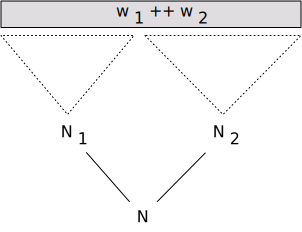
\includegraphics[width=0.5\textwidth]{ChomskyInductionIntuition}
	\caption{The intuition of the Chomsky induction}
	\label{fig:induction}
\end{figure}

To put it more formally: 
\begin{lemma} \label{lemma:chomskyind1}
Let $G$ be a grammar in CNF. Consider an arbitrary nonterminal $N \in G$ and phrase which consists only of terminals $w$. 
If $w$ is derivable from $N$ and $|w| \ge 2$, then there exists two nonterminals $N_1, N_2$ and two phrases $w_1, w_2$ such that: $N \to N_1 N_2 \in G$, $der(G, N_1, w_1)$, $der(G, N_2, w_2)$, $|w_1| \ge 1$, $|w_2| \ge 1$ and $w_1 ++ w_2 = w$.
\end{lemma}


\textbf{Proof.}
The proof heavily uses the fact that grammar $G$ is in CNF in sense of definition given in the work of Gert Smolka and Jana Hofmann.
We apply the hypothesis ``syntactic analysis is possible''. After their application, we get the fact that word $w$ is either a RHS of a rule of grammar $G$, or there is a phrase $phr$, such that (1) word $w$ is derivable from phrase $phr$ and (2) there exists a non-terminal $N$ such that $N \to prh \in G$.

The first case is proved by contradiction since the grammar is in CNF and there might be only a single terminal in a RHS (by assumption we have $|w| \ge 2$).
On the other hand, if there is an intermediate phrase that was obtained by applying a rule, then the phrase has form $N_1 N_2$, since it is also derived by a rule in normal form.
Finally, now we need to prove that both of this nonterminals has a non-empty contribution to the word $w$. This is also true since it is impossible to derive the empty word in CNF grammar (see ~\ref{sec:solka-generalized}).

\begin{lemma}
	Let $G$ be a grammar in CNF. And $P$ be a predicate on nonterminals and phrases (i.e. $P: var \to \textit{phrase} \to \textit{Prop}$).
	Let's also assume that the following two hypotheses are satisfied:
	(1) for every terminal production (i.e. in the form $N \to a$) of grammar $G$, $P(r, [Ts \ r])$ holds and (2) for every $N, N_1, N_2 \in G$ and two phrases that consist only of terminals $w_1, w_2$, if $P(N_1, w_1)$, $P(N_2, w_2)$, $der(G, N_1, w_1)$ and $der(G, N_2, w_2)$ then $P(N, w_1 ++ w_2)$.
	Then for any nonterminal $N$ and any phrase consisting only of terminals $w$, the fact that $w$ is derivable from $N$ implies $P(N,w)$.
\end{lemma}

\textbf{Proof.} 
Let $n$ be an upper bound of the length of word $w$. We carry out the proof by induction on $n$.

\underline{\textit{Base case:}} $ n = 0 $. Proof by contradiction. $|w| \le 0$ implies that $w$ is empty. But an empty word cannot be derived in CNF grammar (see ~\ref{sec:solka-generalized}).

\underline{\textit{Induction step:}} $|w| \le n+1$. This fact is equivalent to the following:  $|w| = n+1$ or $|w| < n$. 
In case of $|w| < n$ we use the induction hypothesis.
Next we consider two new cases, either $|w| = 1 $, or $1 < |w| = n + 1$.
In the first case, it is clear that this is possible only if there is a production $N \to w$, which means one can apply assumption (1).
If the word is longer than 1, then we apply the previous lemma and conclude that $\exists w_1 \ w_2, w = w_1 ++ w_2$. After that,
one need to apply assumption (2). All the generated subgoals are also guaranteed by the lemma ~\ref{lemma:chomskyind1}. 
For shorter words $w_1$ and $w_2$, we apply the induction hypothesis.

\subsection{Intersection of CFG and Automaton}

Since we already have lemmas about the transformation of a grammar to CNF and the transformation of a DFA to a DFA with exactly one state, further we assume that we only deal with (1) DFA with exactly one final state---\textit{dfa} and (2) grammar in CNF---$G$. In this section, we describe the proof of the lemma that states that for any grammar in CNF and any automaton with exactly one state there is a grammar for an intersection of the languages.

\subsubsection{Construction of Intersection}

We present the adaptation of the algorithm given in~\cite{beigelproof}. 

Let $G_{INT}$ be the grammar of intersection. In $G_{INT}$, nonterminals are presented as triples $(\textit{from} \times var \times to) $ where \textit{from} and $to$ are states of \textit{dfa}, and \textit{var} is a nonterminal of $G$.

Since $G$ is a grammar in CNF, it has only two types of productions: $(1)\ N \to a $ and $(2) \ N \to N_{1} N_{2}$, where $N, N_1, N_2$ are nonterminals and $a$ is a terminal.

For every production $N \to N_1 N_2$ in $G$ we generate a set of productions of the form $$(from, N, to) \to (\textit{from}, N_1,  m) (m, N_2, to)$$ where: $from$, $m$, $to$ enumerate all $\textit{dfa}$ states.

\begin{listing}[h]
    \begin{pyglist}[language=coq, numbers=none, numbersep=5pt]
  Definition convert_nonterm_rule_2 
    (r r1 r2: _) 
    (state1 state2 : _) :=
    map (fun s3 => R (V (s1, r, s3)) 
                     [Vs (V (s1, r1, s2)); 
                      Vs (V (s2, r2, s3))])
      list_of_states.

  Definition convert_nonterm_rule_1  
               (r r1 r2: _) 
               (s1 : _) :=
    flat_map (convert_nonterm_rule_2 r r1 r2 s1) 
             list_of_states.

  Definition convert_nonterm_rule (r r1 r2: _) :=
    flat_map (convert_nonterm_rule_1 r r1 r2) 
             list_of_states.
    \end{pyglist}
    \caption{Grammar conversions for nonterminal rules}
    \label{lst:verbments1}
\end{listing}

For every production of the form $N \to a$ we add a set of productions $$(\textit{from}, N, (\textit{dfa\_step}(\textit{from}, a))) \to a$$ where $\textit{from}$ enumerates all $\textit{dfa}$ states and $\textit{dfa\_step (from, a)}$ is the state in which the $\textit{dfa}$ appears after receiving terminal $a$ in the state $\textit{from}$.

\begin{listing}[h]
    \begin{pyglist}[language=coq, numbers=none, numbersep=5pt]
  Definition convert_terminal_rule 
              (next: _) 
              (r: _) 
              (t: _): list TripleRule :=
    map (fun s1 => R (V (s1, r, next s1 t)) 
	               [Ts t]) 
        list_of_states.
    \end{pyglist}
    \caption{Grammar conversion for terminal rule}
    \label{lst:verbments1}
\end{listing}

Next, we join the functions above to get a generic function that works for both types of productions. 
Note that since the grammar is in CNF, the third alternative can never be the case.

\begin{listing}[h]
    \begin{pyglist}[language=coq, numbers=none, numbersep=5pt]
  Definition convert_rule (next: _) (r: _ ) :=
    match r with
    | R r [Vs r1; Vs r2] => 
        convert_nonterm_rule r r1 r2
    | R r [Ts t] => 
        convert_terminal_rule next r t 
    | _  => []   (* Never called *)
    end.
        
  Definition convert_rules 
    (rules: list rule) (next: _): list rule :=
    flat_map (convert_rule next) rules.
    
  (* Maps grammar and s_dfa 
     to grammar over triples *)
  Definition convert_grammar grammar s_dfa :=
    convert_rules grammar (s_next s_dfa). 
    \end{pyglist}
    \caption{Grammar conversion by using rules conversions}
    \label{lst:verbments1}
\end{listing}

Note that at this point we do not conduct any manipulations with the start nonterminal. Nevertheless, the hypothesis of the uniqueness of the final state of the DFA helps to unambiguously define the start nonterminal of the grammar of intersection. The start nonterminal for the intersection grammar is the following nonterminal: \textit{(start, S, final)} where: \textit{start}---the start state of DFA, \textit{S}---the start nonterminal of the initial grammar, and \textit{final}---the final state of DFA. Without the assumption that the DFA has only one final state it is not clear how to unequivocally define the start nonterminal over the alphabet of triples.

\subsubsection{Correctness of Intersection}
\label{sec:correctintersection}

In this subsection we present a high-level description of the proof of correctness of the intersection function.

In the interest of clarity of exposition, we skip some auxiliary lemmas and facts like that we can get the initial grammar from the grammar of intersection by projecting the triples back to the corresponding terminals/nonterminals. Also note that grammar remains in CNF after the conversion, since the transformation of rules does not change the structure of them, but only replaces their terminals and nonterminals with attributed ones.

Next we prove the following lemmas. First, the fact that a word can be derived in the initial grammar and is accepted by \textit{s\_dfa} implies it can be derived in the grammar of the intersection. And the other way around, the fact that a word can be derived in the grammar of the intersection implies that it is derived in the initial grammar and is accepted by \textit{s\_dfa}.

Let $G$ be a grammar in CNF. In order to use Chomsky Induction we also assume that syntactic analysis is possible. 


% Theorem der_in_initial_grammar_and_dfa_implies_der_in_triple_grammar:
%   forall (next: dfa_rule) (r: var) (from to: DfaState) (word: _),
%     der G r (to_phrase word) ->
%     final_state next from word = to ->
%     der (convert_rules G next) (V (from, r, to)) (to_phrase word).
\begin{theorem}
    Let \textit{s\_dfa} be an arbitrary DFA, let $r$ be a nonterminal of grammar $G$, let $from$ and $to$ be two states of the DFA. We also pick an arbitrary word---$w$. If it is possible to derive $w$ from $r$ and the \textit{s\_dfa} starting from the state $from$ finishes in the state $to$ after consuming the word $w$, then the word $w$ is also derivable in grammar \textit{(convert\_rules G next)} from the nonterminal \textit{(V (from, r, to))}.
\end{theorem}

\textbf{Proof.}
It is tempting to use induction on the derivation structure in grammar $G$. But we cannot do it, otherwise we get a phrase (list of terminals and nonterminals) instead of a word. Therefore we should use another way to employ induction, and for the grammar in Chomsky normal form it is possible, as we show in the section~\ref{sec:chomsky-induction}. Roughly speaking, we can split the word into two subwords, such that each of them can be derived from some nonterminal and these two nonterminals is a RHS of some rule from the given grammar.

Let's apply Chomsky induction principle with the following predicate $P$:
\begin{align*}
  P :=  \lambda \ r \ & phr \Rightarrow \\
        &\forall (\textit{next : dfa\_rule}) (\textit{from to : DfaState}), \\
        &\textit{final\_state next from (to\_word phr) = to} \to \\
        &\textit{der (convert\_rules G next, (from, r, to), phr}.
\end{align*}

Basically, predicate $P$ is the property that we are trying to prove in the theorem. Chomsky Induction has 3 assumptions.
(1) The phrase to which $P$ is applied should consist of only non-terminals. We consider only words in this theorem, therefore after conversion of the word to the phrase, no terminals can appear in it. So, we do not violate this assumption.
Moreover, there is a base of induction (2) in the form of a property for a terminal rule and (3) an induction step for a non-terminal rule.
Both statements can be proved by induction on the number of rules in the grammar $G$ in combination with a simple calculation of the functions \textit{convert\_terminal\_rule} and \textit{convert\_nonterm\_rule} for terminal and non-terminal rules, respectively.

On the other side, now we need to prove the theorems of the form  ``if it is derivable in the grammar of triples, then it is accepted by the automaton and is derivable in the initial grammar''.

We start with the DFA.
%          Lemma der_in_triple_grammar_implies_dfa_accepts:
%            forall var word,
%              der (convert_rules G next) (V (from, var , to)) (to_phrase word) ->
%              final_state next from word = to.

\begin{theorem}
	Let \textit{from} and $to$ be states of the automaton, \textit{var} be an arbitrary nonterminal of $G$. We prove that if a word $w$ is derived from the nonterminal \textit{(from, var, to)} in the grammar \textit{(convert\_rules G)}, then the automaton starting from the state \textit{from} consumes the word $w$ and stops in the state $to$.
\end{theorem}

\textbf{Proof.} 
We use the principle of Chomsky Induction.
We apply the induction with the following parameter $P$:

\begin{align*}
P :=  \lambda & \ \textit{tr\_non} \ phr \Rightarrow  \\
              & \textit{final\_state} \textit{\ next \ ($fst_3$ tr\_non) (to\_word \ phr) = $thi_3$ r}. 
\end{align*}

Note that in this case, one need to use projections from attributed nonterminals to simple nonterminals. Induction is carried out in the grammar over triples, but the property operates with the automaton. However, this property can also be expressed in terms of nonterminals-triples.
$P$ is the statement we want to prove.
After applying the induction principle, it remains to prove only the fidelity of the assumptions.
First of all, since $ w $ is a word, converting it to a phrase does not add any nonterminals.
Next, one need to show that the grammar \textit{convert\_rules \ G} is in CNF. It is easy to see, since $G$ in CNF and transformation \textit{convert\_rules} maps symbols in the rules to the symbols over the alphabet of triples.
Finally, one need to show that both assumptions of the induction principle hold.  
In this case it would be: 
\begin{align*}
& (N \to a) \in \textit{convert\_rules} \ G \to \ \ \ \ \ \ \ \ \ \ \ \ \ \ \ \ \ \ \ \ \ \ \ \\
& next (\textit{ $fst_{3}$ } \ (\textit{ unVar } \ N)) \ a = \textit{$thi_3$} \ (\textit{unVar} \ N) 
\end{align*}
and 
\begin{align*}
& (N \to [N_1; N_1]) \in \textit{convert\_rules} \ G  \to \\
& \ \ \ \ \ \ \ \ \ \ \ \ \ \ \ \ \ \ \ \ \ \ \ \ \ \ \ \ \ \ \ \ \ \ \ \ \ \ \ \ \ \ \ \ \ \ \ \ \ \ \ ... \to \\
& \textit{final\_state} \ \textit{next} \ (fst_3 (unVar N)) (to\_word (w_1 ++ w_2)) = \\
& \ \ \ \ \ \ \ \ \ \ \ \ \ \ \ \ \ thi_3 (unVar N)
\end{align*}

In both cases, the proof can be done by an ``inverse'' calculation of functions \textit{convert\_terminal\_rule} and \textit{convert\_nonterm\_rule}. 
That is, by inversing the assumption $$ (N \to [N_1; N_2]) \in \textit{convert\_rules} \ G$$, we gradually come to the conclusion that the only possible option is that the input satisfies the property of the goal. Then it remains to simplify assumptions and conclusion.


Next, we prove the similar theorem for the grammar.

%          Lemma der_in_triple_gr_implies_der_in_initial_gr:
%            forall (s_start s_final: DfaState) (grammar_start: _) (word: word),  
%              der (convert_rules G next) (V (s_start, grammar_start, s_final)) (to_phrase word) ->
%              der G grammar_start (to_phrase word).
\begin{theorem}
	Let \textit{from} and $to$ be the states of the automaton, let \textit{var} be an arbitrary non-terminal of grammar G. We prove that if a word $w$ is derivable from the nonterminal \textit{(from, var, to)} in the grammar \textit{(convert\_rules G)}, then $w$ is also derivable in the grammar $G$ from the nonterminal \textit{var}.
\end{theorem}

\textbf{Proof.} 
We again prove the theorem using Chomsky induction with the following predicate $P$:
\begin{align*}
P :=  \lambda \ r \ phr \Rightarrow \textit{der(G, $snd_3$ (unVar r), phr)}.
\end{align*}

Note that the induction is carried out in the grammar over triples, but the property is about the ``unit'' grammar, therefore we use projections from triples to non-triples.
Here we can use the same idea of ``inversing'' of functions \textit{convert\_terminal\_rule} and \textit{convert\_nonterm\_rule}.
By inversing the induction hypothesis, we gradually come to the conclusion that the only possible option is that the input satisfies the property of the goal. 

%R (V (from, r, to)) [Ts t] el convert_rules G next -> R r [Ts t] el G. 
%И аналогично для нетерминальных правил, только начиная с правила вида ... можно получить ... 
%R (V (from, r, to)) [Vs (V (from1, r1, to1)); Vs (V (from2, r2, to2))] el convert_rules G next -> R r [Vs r1; Vs r2] el G.
 


Well, in the end one need to combine both theorems to get full equivalence. By this, the correctness of the intersection is proved.

\subsection{Union of Languages}

During the previous step we constructed a list of context-free grammars. In this section, we provide a function which constructs a grammar for the union of the languages.

First, we need to make sure the sets of nonterminals for each of the grammars under consideration have empty intersections. To achieve this, we label nonterminals. Each grammar of the union receives a unique ID number and all nonterminals within one grammar will have the same ID as the grammar. In addition, it is necessary to introduce a new start nonterminal of the union.

\begin{listing}[h]
    \begin{pyglist}[language=coq, numbers=none, numbersep=5pt]
  Inductive labeled_Vt : Type :=
  | start : labeled_Vt
  | lV : nat -> Vt -> labeled_Vt.
  
  Definition label_var (label: nat) 
                       (v: @var Vt): @var 
                       labeled_Vt :=
    V (lV label v).  
    \end{pyglist}
    \caption{Definitions of labeled type and labeling function}
    \label{lst:verbments1}
\end{listing}

The function that constructs the union grammar~(Lst.\ref{lst:grm-union}) takes a list of grammars, then, it (1) splits the list into head [$h$] and tail [$tl$], (2) labels [\textit{length \ tl}] to $h$, (3) adds a new rule from the start nonterminal of the union to the start nonterminal of the grammar [$h$], finally (4) the function is recursively called on the tail [$tl$] of the list.

\begin{listing}[h]
    \begin{pyglist}[language=coq, numbers=none, numbersep=5pt]
  Definition label_grammar label grammar := ...

  Definition label_grammar_and_add_start_rule 
               label 
               grammar :=
    let '(st, gr) := grammar in 
    (R (V start) [Vs (V (lV label st))]) 
       :: label_grammar label gr.        

  Fixpoint grammar_union 
     (grammars : seq (@var Vt * (@grammar Tt Vt)))
       : @grammar 
     Tt 
     labeled_Vt :=
    match grammars with
    |  [] => []
    |  (g::t) => 
         label_grammar_and_add_start_rule 
           (length t) 
           g ++ (grammar_union t)
    end.
    \end{pyglist}
    \caption{Grammars union and helper functions}
    \label{lst:grm-union}
\end{listing}

\subsubsection{Proof of Languages Equivalence}

In this section, we prove that the function \textit{grammar\_union} constructs a correct grammar of the union language. Namely, we prove the following theorem.

\begin{theorem} \label{theorem-correct-union}
    Let \textit{grammars} be a sequence of pairs of starting nonterminals and grammars. Then for any word $w$, the fact that $w$ belongs to the language of union is equivalent to the fact that there exists a grammar $(st,gr) \in \textit{grammars}$ such that $w$ belongs to the language generated by $(st,gr)$.
\end{theorem}

\begin{listing}[h]
    \begin{pyglist}[language=coq, numbers=none, numbersep=5pt]
  Variable grammars: seq (var * grammar).

  Theorem correct_union:
    forall word, 
      language (grammar_union grammars) 
        (V (start Vt)) (to_phrase word) <->
      exists s_l, 
        language (snd s_l) (fst s_l) 
          (to_phrase word) /\ 
        In s_l grammars.
    \end{pyglist}
    \caption{Theorem on languages equivalence}
    \label{lst:lang-eq}
\end{listing}


\textbf{Proof of theorem~\ref{theorem-correct-union}.} Since the statement is formulated as an equivalence, we divide the proof into two parts.
\begin{enumerate}
\item If $w$ belongs to the union language, then $w$ belongs to one of the initial languages. \\
From an auxiliary lemma, we know that either (1) the phrase is equal to the starting nonterminal or (2) there exists a grammar $G$ from the grammars-list such that the phrase is derivable from the labeled starting nonterminal of grammar $G$.
Let us prove that this is the grammar we are interested in.
Since we consider the word, it cannot be the start nonterminal. So this might be only the second case.
According to another lemma, if the output does not start from the start nonterminal, then it cannot appear in this derivation. So all the rules that use the start nonterminal can be safely (for this derivation) removed from the grammar.
There is a lemma that says, that a derivation that starts from a nonterminal labeled by $x$ cannot contain any nonterminals with a label other than $x$. Therefore, for this derivation, one can ignore the rules with other labels.
These two grammars are identical, but one of them is labeled and the other is not. It is clear that if there exists a bijection between nonterminals the set of derivable words does not change.

\item If $w$ belongs to one of the initial language, then $w$ belongs to the union language. \\
In this case, one explicitly specify the corresponding derivation in the union-grammar.
The labeling function is arranged in such a way that knowing the place of a certain grammar in the list of grammars, one can calculate the exact number that will be assigned to this grammar as a label.
After that proof can be finished in two steps. 
\begin{enumerate}
\item One need to apply the rule from the start nonterminal of the union-grammar to the start nonterminal of the initial grammar. 
\item One should use the fact that derivation in the initial grammar and the labeled grammar are equivalent.
\end{enumerate}
\end{enumerate}

\subsection{Putting All Parts Together}

Now we can put all previously described lemmas together to prove the main statement of this paper.

\begin{listing}[h]
    \begin{pyglist}[language=coq, numbers=none, numbersep=5pt]

Theorem grammar_of_intersection_exists:
  exists 
   (NewNonterminal: Type) 
   (IntersectionGrammar: 
      @grammar Terminal NewNonterminal) St,
  forall word,
    dfa_language dfa word /\ 
	    language G S (to_phrase word) <->
    language IntersectionGrammar St 
	         (to_phrase word).
   \end{pyglist}
\caption{Final theorem}
\label{lst:lang-eq}
\end{listing}

\begin{theorem}
    For any two decidable types $Tt$ and $Nt$ for type of terminals and nonterminals correspondingly.
    If there exists a bijection from $Nt$ to $\mathbb{N}$ and syntactic analysis in the sense of definition~\ref{lst:synt-analysis-is-possible} is possible, then for any DFA \textit{dfa} that define language over $Tt$ and any context-free grammar $G$, there exists the context-free grammar $G_{INT}$ , such that $L(G_{INT}) = L(G) \cap L(\textit{dfa})$.
\end{theorem}   

\textbf{Proof.} 
Let $NG$ be the grammar in CNF obtained after applying the algorithm of~\cite{smolkaHofmann2016}. Let \textit{sdfas} be the list of DFAs with exactly one final state obtained after splitting \textit{dfa}.
Since we now have $NG$ in CNF and the list of DFAs with one state, we can compute a list of their intersections.
I.e. we intersect each of the \textit{sdfa} of the list with the grammar $NG$.
Next, we find the union of the languages. 

Next, we divide the proof into two branches.
We check whether the empty word is accepted by the \textit{dfa} and is derived in the grammar $G$.
(1) If so, we add one more rule to the language of the union ($ S \to \varepsilon$). (2) If not, we add nothing.

Now for the cases (1) and (2) we prove that $G_{INT}$ is the grammar of the intersection.
That is, if a word is accepted by the \textit{dfa} and is derivable in $G$, then it must also be derivable in $G_{INT}$ and vice versa.

For branch (1) we carry out the proof in 2 stages.

\begin{enumerate}
\item[a] Consider the case when $w$ is an empty word.
By assumption, we already know that the empty word is accepted by the DFA and can be derived in the grammar. But we also know that we have added a rule from the start nonterminal to the empty word to the grammar of the intersection. So, if $w$ is an empty word it derivable in both cases.
\item[b] Let's now prove for the case when $w$ is non-empty.
We consistently modify the premises and the conclusion using theorems about equivalences. First we prove that the fact that $w$ derivable in $G$ and is accepted by \textit{dfa} implies the fact that $w$ is also derivable in $G_{INT}$. We can safely remove the rule $S \to \varepsilon$, since we apply the unification only to grammars in CNF (any grammar of intersection is in CNF), the epsilon rule cannot be used anywhere except for the initial step.
Since the word is accepted by \textit{dfa}, then there is a DFA with one final state \textit{sdfa}, which also accepts this word. So, we can safely replace \textit{dfa} with \textit{sdfa}. 
For grammar $G$ there is a equivalent grammar $NG$ in CNF. Since word $w$ is not empty, we maintain equivalence.
Let $INT$ be a grammar of the intersection of \textit{sdfa} and $NG$. We can use theorems from section~\ref{sec:correctintersection} to prove that it is a grammar of the intersection of \textit{sdfa} and $G$. 
But by the construction, such a grammar belongs to the union of languages $G_{INT}$. This finishes inclusion of $G$ and \textit{sdfa} to $G_{INT}$.
In the other direction: the fact that $w$ is derivable in $G_{INT}$ implies that $w$ is derivable in the grammar $G$ and is accepted by the DFA \textit{dfa}. 
\end{enumerate}

Grammar $G_{INT}$ consists of a union of the empty language and list languages of the intersection of some DFA with one final state and grammar in CNF. We can safely remove an empty grammar since $w$ is not an empty word and any grammar in the list of languages of the intersection is in CNF.
We know that since the word is accepted by $G_{INT}$ grammar, there is a grammar from the union of grammars in which this word is derivable.
But this grammar is a grammar of intersection of some DFA with one final state and grammar in CNF. Now we can use theorems from section~\ref{sec:correctintersection} to prove equivalence.

The second case is when the empty word is not derivable in $G$ and is not accepted by \textit{dfa}.
For an empty word, one needs to prove that it is not derivable in the grammar of the intersection. 
None of the grammars from the union has the rule $S \to \varepsilon$. 
Next, one has to repeat what is discussed above, but without the additional steps about the empty language.
 	